\section{作成したシステムの概要}
本システムは，1台のサーバと4台のクライアントから構成される分散型の自動演奏システムである．
サーバとクライアントにはいずれもArduinoを用いる．サーバは楽曲全体のテンポを管理する指揮者としての役割を担い，
各クライアントはピアノ，トロンボーン，カスタネット，バイオリンのいずれか1つの楽器を担当する奏者として動作する．
サーバとクライアントは同一のWi-Fiネットワークに接続され，サーバはテンポと小節番号をUDPローカルブロードキャストによって
全クライアントへ一斉送信する．

本システムは通信・同期機能，楽器音源の生成・再生機能，人形の物理演出機能の3つの機能から構成される．
通信・同期機能は，サーバが送信する小節番号とテンポをクライアントが受信し，演奏のタイミングを制御する機能である．
楽器音源の生成・再生機能は，クライアントが受信した小節番号から演奏する音符を決定し，シリアル通信を介して
PC上のProcessingへ送信することで音源を再生する機能である．人形の物理演出機能は，クライアントが受信した
小節番号に基づいてサーボモータを駆動し，演奏に同期した人形の動作を行う機能である．
報告者は，このうち楽器音源の生成・再生機能，および人形の物理的な製作を担当した．
本節では，まずシステム全体の構成と信号の流れを示し，続いて各機能について説明する．

\subsection{システム全体の構成}
% 構成図（サーバ1台＋クライアント複数）と，各クライアントの担当楽器・人形の対応，信号の流れを図で示す
\subsection{システム全体の構成}
本システムの全体構成を図\ref{fig:overview}に示す．サーバと4台のクライアントは同一のWi-Fiネットワークに接続される．
サーバは楽曲のテンポと演奏中の小節番号を管理し，これらをUDPローカルブロードキャストによって全クライアントへ
一斉に送信する．各クライアントには演奏する楽曲の譜面データがあらかじめ保持されており，受信した小節番号に対応する
音符を譜面データから読み出す．

\begin{figure}[h]
    \centering
    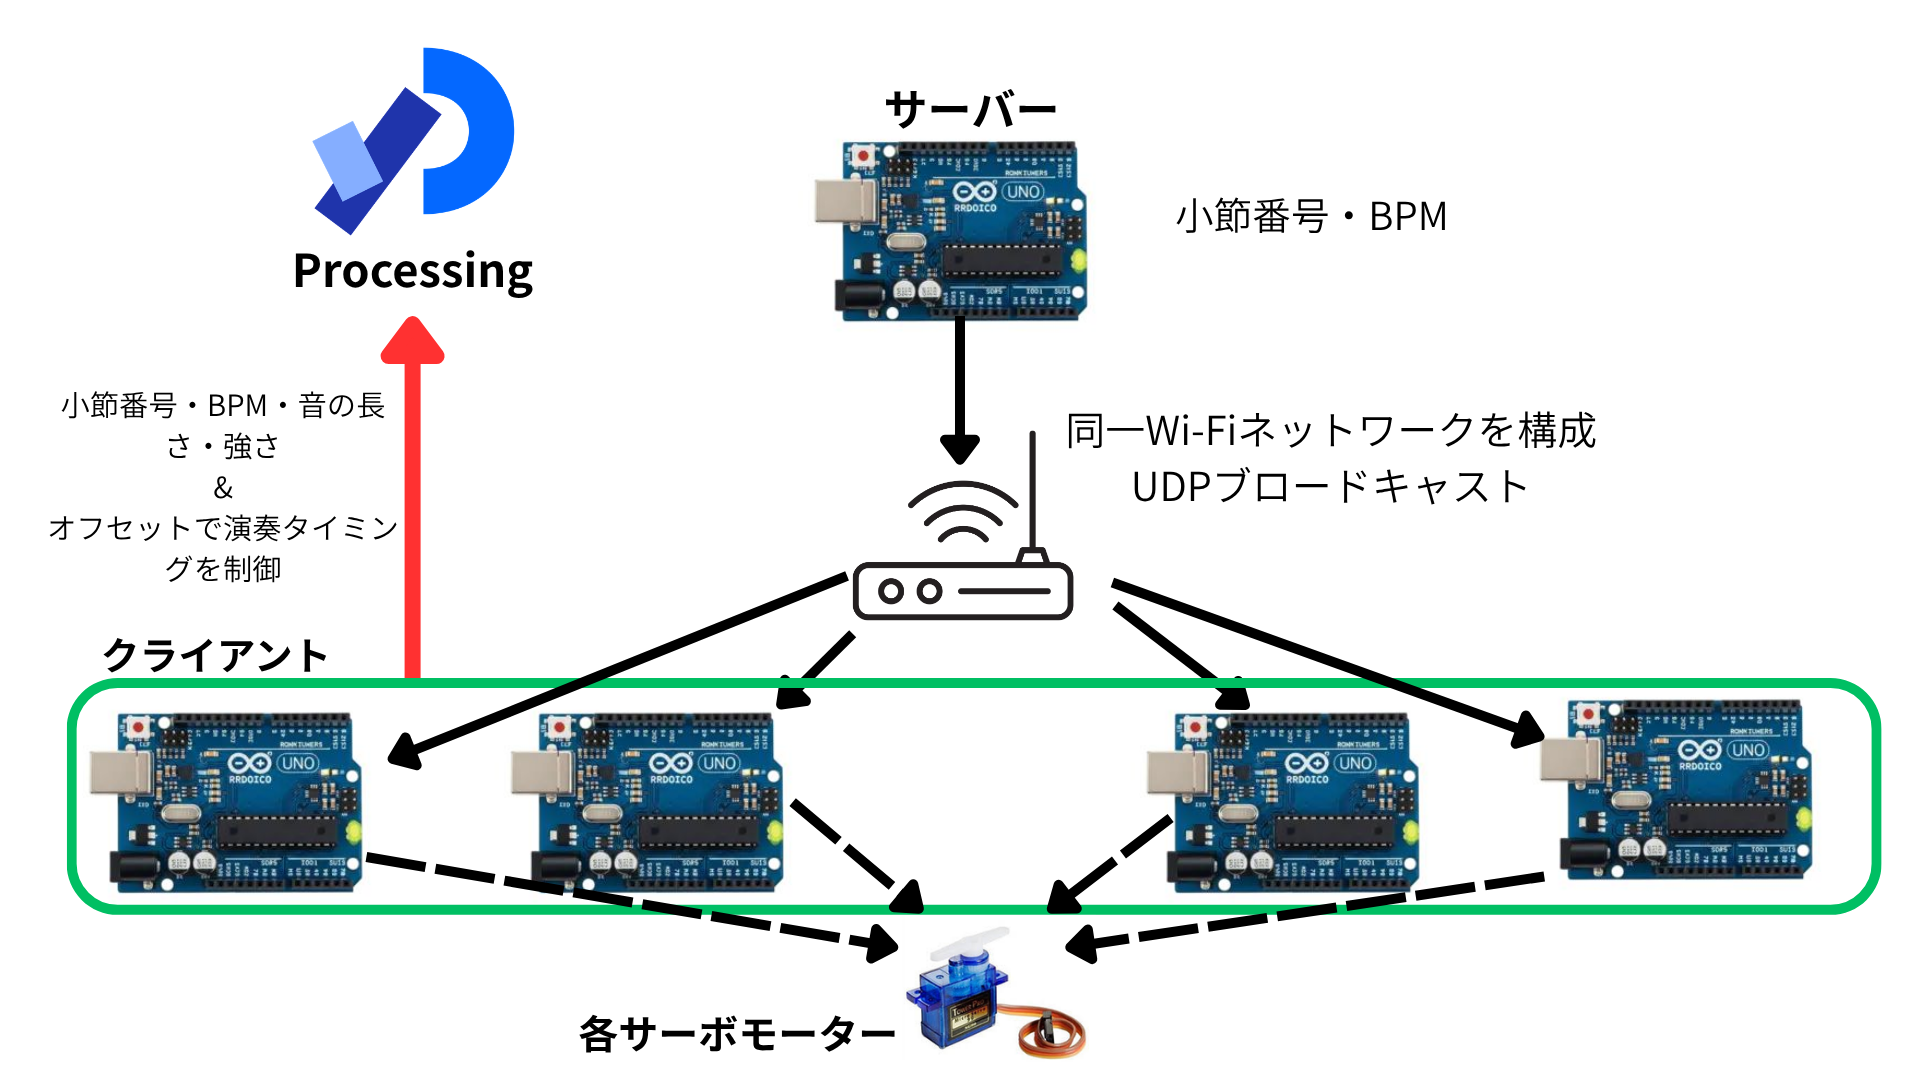
\includegraphics[width=0.8\linewidth]{fig/システム全体構成図.png}
    \caption{システム全体の構成}
    \label{fig:overview}
\end{figure}

各クライアントが担当する楽器の発音は，クライアントに接続されたPC上のProcessingが行う．各クライアントは，
譜面データから読み出した音符の周波数，発音する長さ，強さ，およびテンポをシリアル通信によってProcessingへ送信する．
Processingは受信した情報をもとに楽器音源を合成し，スピーカから再生する．このように，サーバからクライアントへは
Wi-Fiを介して小節番号とテンポが送信され，各クライアントからProcessingへはシリアル通信を介して個々の音符の情報が
送信されるという二段階の信号の流れによって，システム全体の演奏が実現される．
また，各クライアントは受信した小節番号に基づいてサーボモータを駆動し，演奏に同期した人形の動作を行う．

\subsection{通信・同期機能}
% 1章の独自性に対応する中核。サーバ：BPMから小節タイミング算出→UDPブロードキャスト／
% クライアント：受信→内部タイマで自律補間／1バイトのバイナリ設計／再送なしのフェイルセーフ
% ※原理・方式レベルで。コードや閾値などの実装詳細は3節へ
通信・同期機能は，サーバが送信する演奏位置とテンポの情報をクライアントが受信し，各クライアントの演奏の
タイミングを制御する機能である．同期通信の構成を図\ref{fig:sync}に示す．サーバには2つのスイッチが接続されており，
一方を押すとテンポが増加し，他方を押すとテンポが減少する．これにより，演奏中にテンポをリアルタイムで変更できる．
サーバは，現在のテンポと演奏中の小節番号を1バイトのデータとしてUDPでブロードキャストする．クライアントは
受信したデータの値によってその種別を判別し，一定値以上であればテンポ，それ未満であれば小節番号として扱う．
\begin{figure}[h]
    \centering
    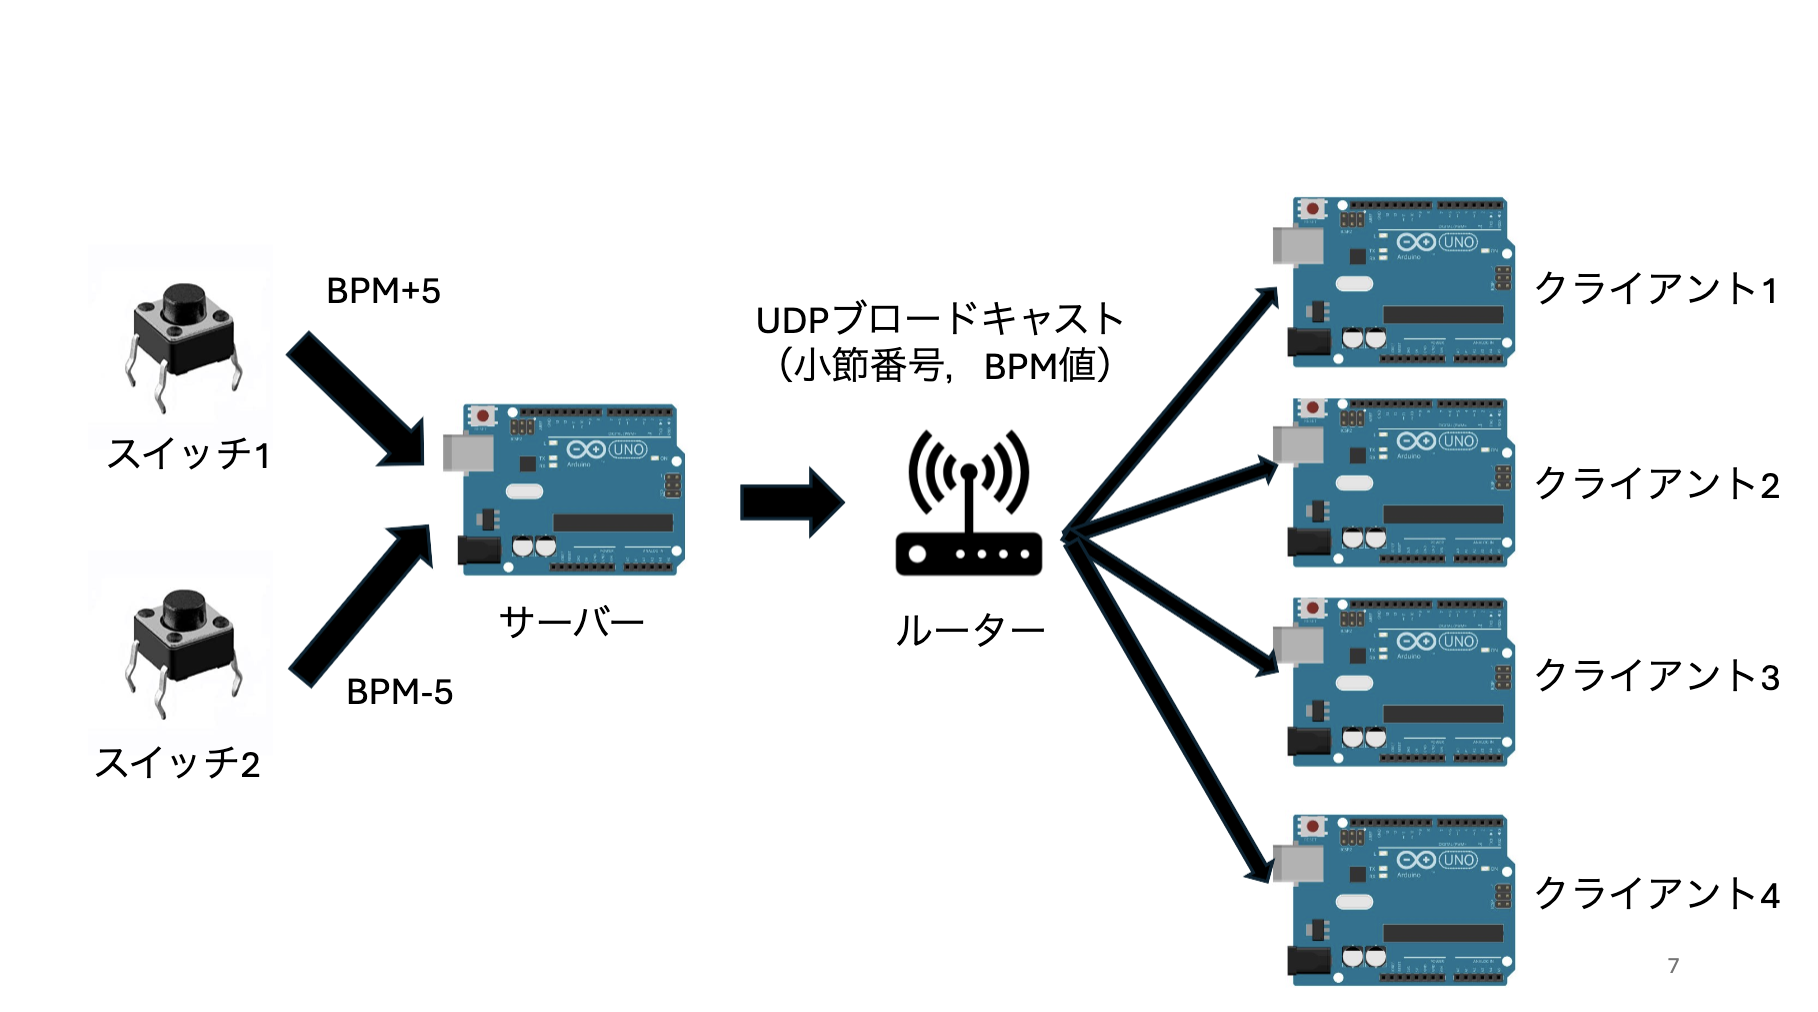
\includegraphics[width=0.8\linewidth]{fig/通信構成図.png}
    \caption{同期通信の構成}
    \label{fig:sync}
\end{figure}

テンポを受信したクライアントは，そのテンポから基準となる4分音符の長さを算出し，以降の演奏の時間基準とする．
小節番号を受信したクライアントは，あらかじめ保持している譜面データからその小節に含まれる音符を先頭から順に
読み出し，各音符の相対的な長さと基準音符長から求めた間隔で，音符の情報をProcessingへ順次送信する．
これにより，サーバが小節単位の位置情報のみを送信し，各クライアントが自身のもつ譜面データに基づいて
小節内の演奏を自律的に進める構成となっている．

また，各クライアントは輪唱を実現するためのオフセットを保持しており，受信した小節番号にオフセットを加えることで
自身の演奏開始位置をずらす．これにより，同一の譜面を複数のクライアントが時間差で演奏し，輪唱として
成立させている．

\subsection{音源の生成・再生機能}
% トロンボーン：波形合成による音色・音階の生成／カスタネット：打楽器音の波形と特有のノイズ
% ※詳細（波形・周波数の実測など）は3節・4節へ
楽器音源の生成・再生機能は，クライアントから送信された音符の情報をもとに，PC上のProcessingが楽器の音を
合成して再生する機能である．Processingは，クライアントからシリアル通信で受信した周波数，発音する長さ，強さ，
およびテンポを解釈し，指定された周波数の音を，その楽器に応じた音色で，指定された長さだけ発音する．

各楽器の音色は，実際の楽器の音響的な特徴を反映するように設計した．例えば，
トロンボーンは音高の明確な持続音を発する楽器であるため，加算合成によって
その音色を再現した．一方，カスタネットは音高を持たない打楽器であり，特定の周波数帯に集中した打撃音を
再現した．これらの音源の具体的な設計と実装については\ref{sec:impl}章で述べる．

\subsection{物理演出機能}
% 人形の駆動機構と，音に同期させる仕組み
物理演出機能は，演奏に合わせて楽器を持った人形を動作させ，視覚的な演出を行う機能である．各クライアントArduinoには
サーボモータが接続されており，人形の腕などの可動部を駆動する．クライアントは，受信した小節番号に基づいて
その小節で演奏すべき動作のタイミングを求め，音の発生に同期してサーボモータを動かす．これにより，人形が
楽器を演奏しているように見せる．

また，各クライアントはテンポの変化を受信した際に，人形に演奏以外の動作を行わせる．これにより，楽曲の
進行に合わせた人形の反応を表現する．人形は演奏する楽器に応じて異なる動作を行い，楽器ごとの演奏の
様子を表現する．ピアノの場合，両手で鍵盤を叩くような動作を行い，トロンボーンの場合は楽器をベルアップさせて下げる動作を繰り返す．
ヴァイオリンは，弓を楽器に当ててさらに口が開くような動作を行い，カスタネットは両手でカスタネットを叩く動作を行う．
カスタネットは，サーバー側のテンポ変化が起きると頭が回転するという動作も行う．